\chapter{Sistemas imunológicos e a Teoria do Perigo}

Uma das funções principais do sistema imunológico é a proteção contra infecções \cite{Cayzer2007}. O reconhecimento de agentes infecciosos é feito através de fragmentos característicos de proteínas chamados de \emph{antígenos}.

A arquitetura do sistema imunológico natural apresenta diversas camadas: um agente patogênico que consiga infiltrar-se no corpo enfrentará os sistemas imunológicos \emph{inato} e \emph{adaptativo}. Esses dois sistemas interrelacionados são constituídos de diversos tipos de moléculas e células, produzidas por órgãos e processos especializados para lidarem com o problema da discriminação do próprio e não-próprio. Essa discriminação é feita no nível mais baixo, com a interação entre as superfícies das células e moléculas e dos agentes patogênicos.

A primeira linha de defesa do corpo é o sistema imunológico inato, que existe desde o nascimento. Esse sistema não gera respostas específicas para cada tipo de invasor. Ele é constituído de proteções básicas como a pele, cílios, lágrimas, saliva e células como os macrófagos, que nautralizam os agentes externos em áreas de infecção.

No entanto, alguns agentes infecciosos são capazes de ultrapassar essas barreiras básicas. Nesse caso, entra em ação o sistema imunológico adaptativo, que recebe esse nome por prover respostas imunológicas específicas para cada tipo de antígeno ao qual é exposto. A resposta imunológica é gerada pela identificação de um agente externo, o que leva à ativação de certa células que removem o agente do corpo. Uma memória de exposições é mantida, e é utilizada quando o mesmo agente infecta o corpo novamente, mostrando um comportamento de aprendizagem na identificação \cite{Brownlee2011}.

A primeira resposta, ou \emph{resposta primária}, é lenta, levando até algumas semanas para remover a infecção. Caso o agente patogênico seja encontrado novamente, ocorre uma \emph{resposta secundária}, onde é aplicado o que foi aprendido na resposta primária, tornando a resposta imunológica mais rápida e eficiente. A memória adquirida tem duração longa, geralmente provendo imunidade por toda a vida do hospedeiro (dois exemplos são varicela e sarampo).

O primeiro modelo do sistema imunológico foi o da distinção entre o próprio e o não-próprio, proposto por \citet{Burnet1959}. Ao longo do tempo, novos modelos foram criados, tentando resolver as questões que os outros modelos não explicavam, destacando-se o modelo do não-próprio infeccioso \cite{Janeway1989}, sendo aceito atualmente como o mais completo pelos imunologistas. As figuras abaixo (\ref{img:signals-first} a \ref{img:signals-last}) mostram a evolução dos modelos, e foram retiradas de \citet{Aickelin2002}.

\section{Discriminação do próprio e não-próprio}

No modelo de disciminação do próprio e não próprio (Self Non-self Discrimination, SNSD) de Burnet, existe apenas um tipo de linfócito, o linfócito B, responsável por identificar os antígenos e produzir os respectivos anticorpos. A resposta imune adaptativa é gerada apenas pela identificação desses antígenos, sem qualquer mecanismo de controle.

\begin{figure}[h!]
\centering
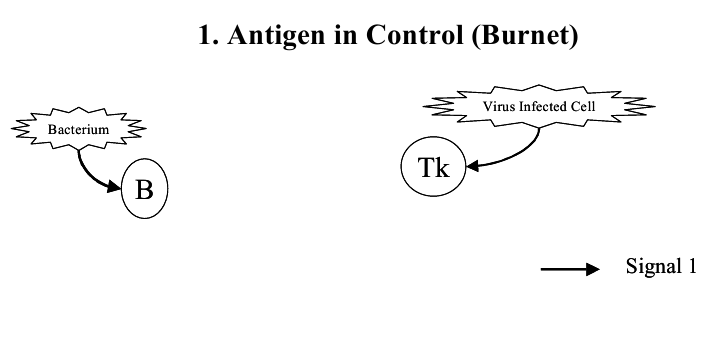
\includegraphics[width=0.75\textwidth]{img/signals1-antigen.png}
\caption{SNSD: Antígeno no controle}
\label{img:signals-first}
\end{figure}

Em algum ponto no início da vida, os linfócitos aprendem a diferenciar o próprio, células pertencentes ao corpo, do não-próprio, células estranhas ao corpo, que devem ser eliminadas. As células que geram respostas auto-imunes (reações contra as células próprias) são removidas nesse ponto, restando apenas as capazes de identificar o não-próprio.

\begin{figure}[h!]
\centering
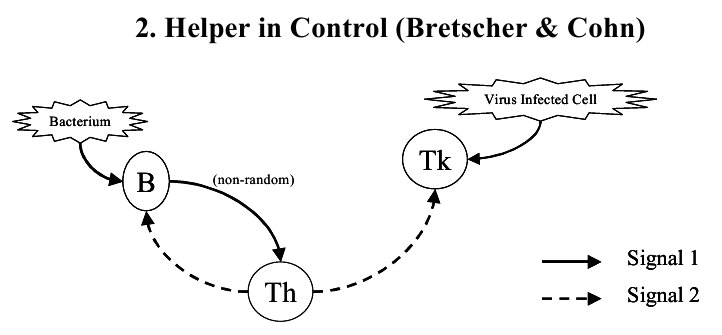
\includegraphics[width=0.75\textwidth]{img/signals2-helper.png}
\caption{Auxiliar no controle}
\end{figure}

Bretscher e Cohn introduziram uma segunda célula, o linfócito T auxiliar, ou T$_{h}$ (T \emph{helper}), que regulava a ativação dos linfócitos B. O linfócito B apresenta o antígeno ao linfócito T e aguarda sua confirmação para iniciar a resposta. A introdução dessa célula tem o objetivo de evitar uma reação auto-imune sem controle. Lafferty e Cunningham introduziram uma terceira célula, a Célula Apresentadora de Antígeno (APC, \emph{Antigen Presenting Cell}), cuja função é decompor os antígenos e apresentá-los aos linfócitos T. Dessa forma, o funcionamento das células do modelo anterior agora depende da ativação do linfócito T pela APC.

\begin{figure}[h!]
\centering
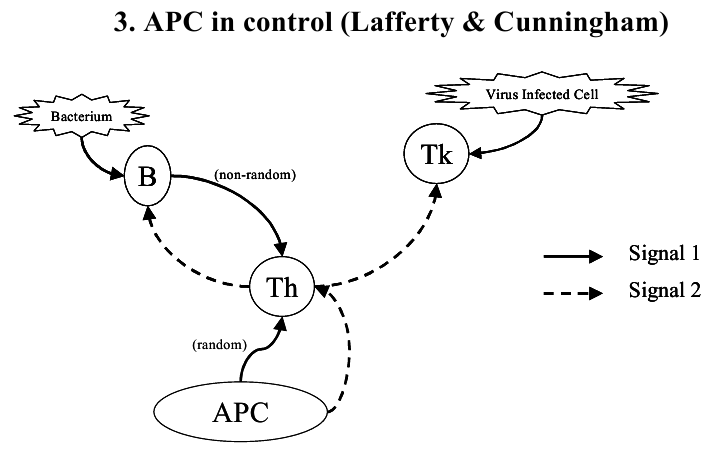
\includegraphics[width=0.75\textwidth]{img/signals3-apc.png}
\caption{APC no controle}
\end{figure}

\section{Não-próprio infeccioso}

O modelo mais aceito na imunologia atualmente, o modelo não-próprio infeccioso (Infectious Non-Self, INS), foi proposto por Janeway \cite{Janeway1989}. Nele, as APCs também têm de ser ativadas: elas só enviam o sinal dois aos linfócitos T quando tiverem reconhecido padrões patológicos no antígeno. Assim, da mesma forma, o funcionamento do modelo anterior depende de um novo fator, antes a APC, agora o reconhecimento de padrões pela APC.

\begin{figure}[h!]
\centering
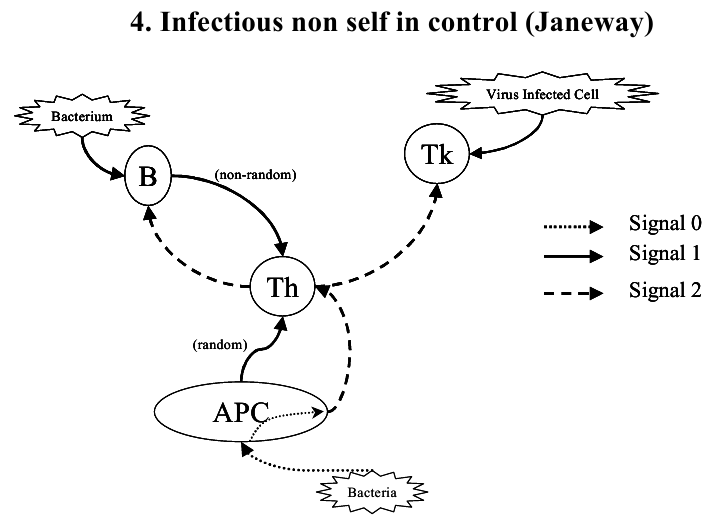
\includegraphics[width=0.75\textwidth]{img/signals4-ins.png}
\caption{INS: Não-próprio infeccioso no controle}
\end{figure}

\section{A Teoria do Perigo}

Uma adição ainda mais recente foi a da Teoria do Perigo \cite{Matzinger1994}. Matzinger defende a teoria de que não é a separação do próprio e do não-próprio a força que impulsiona o sistema imunológico, mas sim o que ela caracteriza como ``perigo'': qualquer coisa que cause estresse ou morte não-apoptética (não natural) da célula. A Teoria do perigo baseia-se em sinais gerados pelos tecidos danificados para diferenciar entre eventos malignos e benignos \cite{Cayzer2007}.

Embora não seja completa, essa teoria explica fenômenos que as teorias baseadas na discriminação do próprio e não-próprio não explicavam, como o fato de não haver reação contra bactérias no intestino ou na comida, a mudança do conceito de próprio durante a vida e a problemática da própria definição do próprio e do não-próprio.

Mais do que isso, a Teoria do Perigo muda a forma como se enxerga o sistema imunológico como um todo: um sistema responsável por manter o corpo em estado de equilíbrio. Dessa forma, a distinção explícita do próprio se torna desnecessária. Discriminação ainda existe, mas seu foco é o perigo, não mais o estranho.

Uma explicação detalhada do sistema imunológico, e seu funcionamento conforme a Teoria do Perigo, é apresentado na figura 1, abaixo\footnote{MATZINGER, P. \emph{op. cit.}}. Os linfócitos B são os responsáveis pela identificação de antígenos através de receptores em sua superfície. Durante uma infecção, essas células se multiplicam e produzem anticorpos para eliminar os antígenos identificados. Elas são capazes de adaptar-se a virtualmente qualquer tipo de antígeno, gerando a resposta adequada. Um outro tipo de linfócito, os linfócitos T, quando ativados, podem exercer uma de duas funções: os linfócitos T citotóxicos (CTL) são responsáveis pela eliminação de células infectadas, enquanto que os linfócitos T auxiliares (T$_{h}$) são responsáveis pela ativação de outras células, entre elas os linfócitos B.

Além disso, alguns linfócitos T são mantidos como células de memória. Durante a resposta imunológica, os linfócitos B e T$_{h}$ se multiplicam para combater os antígenos, e são removidos quando a resposta termina. No entanto, alguns linfócitos T são mantidos, para que possam ser usados em futuras respostas ao mesmo tipo de antígeno. A combinação de linfóctios T virgens (sem um tipo de antígeno associado) e de memória permite que o sistema imunológico gere respostas tanto a novas ameaças quanto a ameaças recorrentes.

Existe ainda um outro tipo de linfócito, o T \emph{killer} (Tk), que não tem receptores antígeno-específicos, mas é capaz de reconhecer células infectadas e algumas células anormais. O objetivo dessas células é atuar como a primeira defesa contra infecções, e são muito importantes nos começo da vida.

\begin{figure}[h!]
\centering
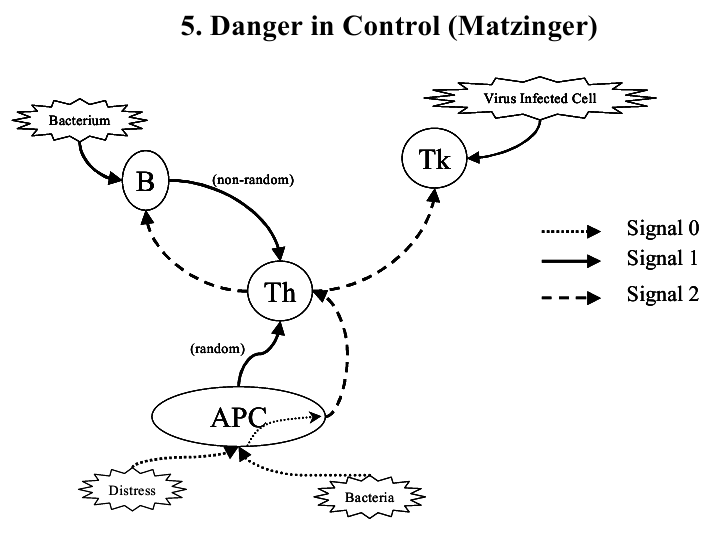
\includegraphics[width=0.75\textwidth]{img/signals5-danger.png}
\caption{Perigo no controle}
\label{img:signals-last}
\end{figure}

O comportamento dos linfócitos T e B se baseia em três regras:

\begin{enumerate}
\item Linfócitos T e B entram em atividade ao receber os sinais um e dois, morrem ao receber apenas o sinal um e ignoram o sinal dois sem o recebimento do sinal um.
\item Linfócitos T aceitam o sinal dois apenas de APCs, enquanto os linfócitos B, apenas de linfócitos T ativos ou células de memória. O sinal um pode ter origem em qualquer célula.
\item Linfócitos T ativados não precisam do sinal dois para entrarem em ação. Após um período de tempo, elas voltam ao estado de repouso, necessitando novamente dos dois sinais.
\end{enumerate}

Células Apresentadoras de Anítgeno (ATP, ou Antigen Presenting Cell) são as células responsáveis por apresentar os antígenos às células T. Essas células podem ser os linfócitos B, macrófagos e as células dendríticas. Quando as células se encontram em estado de estresse ou morrem de forma não programada, enviam um sinal para as células APC, representado pela seta Sinal 0. Isso desencadeia o envio do sinal dois para os linfócitos Th. Enquanto isso, linfócitos B usam seus receptores para reconhecer antígenos nas suas redondezas, enviando o sinal um para os linfócitos Th. É o par de sinais um (reconhecimento do antígeno) e dois (sinal enviado pelo linfócito T, ativado pelo sinal de perigo) que faz com que a reação imunológica tenha início.

Um conceito importante da Teoria do Perigo é a tolerância. Linfócitos B que reconhecem células próprias continuamente recebem o sinal um (identificação através dos receptores em sua superfície). No entanto, essas células não apresentam perigo (não causam danos a outras células), logo o sinal dois nunca será gerado. Pela lei um acima, sem receber o sinal dois de outras células, o linfócito será removido. Dessa maneira, corpos estranhos mas que não causem dano (perigo) ao corpo não geram respostas imunes.

\section{Considerações finais}

A imunologia como ciência existe desde o século 18, e o sistema imunológico ainda é uma grande fonte de pesquisa, em particular a natureza distribuída de seus mecanismos de memória, auto-tolerância e controle descentralizado. Baseando-se no funcionamento do sistema imunológico biológico, foram criados Sistemas Imunológicos Artificiais: algoritmos, estruturas e sistemas computacionais que inspiram-se nos modelos do sistema imunológico. Esses sistemas podem ser usados por imunologistas para explanação, experimentação ou previsão de situações que seriam difíceis ou impossíveis de serem reproduzidas em testes de laboratório \cite{Garrett2005}. Essa técnica é conhecida como ``imunologia computacional''.

No entanto, a maioria dos modelos de Sistemas Imunológicos Artificiais também são utilizados como abstrações dos processos imunológicos para o desenvolvimento de sistemas computacionais. O sistema imunológico é um sistema adaptativo complexo, que evoluiu nos seres vertebrados para protegê-los de invasores. O objetivo do estudo dos Sistemas Imunológicos Artificiais é aplicar no design de sistemas computacionais estruturas e funcionalidades inspiradas nos modelos biológicos. \citeauthor{Dasgupta2006} define a importância dos Sistemas Imunológicos Artificiais da seguinte forma:

\begin{quote}
    Do ponto de vista do processamento de informação, o sistema imunológico é um sistema adaptativo notavelmente paralelizado e distribuído com um mecanismo de controle (parcialmente) descentralizado. Ele usa extração de características, sinalização, aprendizagem, memória e recuperação associativa para solucionar tarefas de reconhecimento e de classificação. Em particular, ele aprende a reconhecer padrões relevantes, lembrar padrões que foram já foram vistos e usar análise combinatória para construir detectores de padrão eficientes. Além disso, o funcionamento do sistema como um todo é uma propriedade emergente de muitas interações locais. Essas notáveis habilidades de processamento de informações do sistema imune representam aspectos importantes no campo da computação. \cite{Dasgupta2006}\footnote{``From an information-processing perspective, the immune system is a remarkable parallel and distributed adaptive system with (partial) decentralized control mechanism. It uses feature extraction, signaling, learning, memory, and associative retrieval to solve recognition and classification tasks. In particular, it learns to recognize relevant patterns, remember patterns that have been seen previously, and use combinatorics to construct pattern detectors efficiently. Also, the overall behavior of the system is an emergent property of many local interactions. These remarkable information-processing abilities of the immune system provide several important aspects in the field of computation.''\cite{Dasgupta2006}}
\end{quote}

Durante a história da Inteligência Artificial, os modelos biológicos inspiraram muitos modelos de algoritmos imunológicos. Tipos diferentes de modelos podem ser utilizados em domínios diferentes de problemas e existem modelos que podem ser aplicados em mais de um domínio. Dentre estes modelos, destacam-se o algoritmos de seleção negativa, as redes imunológicas artificiais, o algoritmo de seleção clonal, os algoritmos genéticos e os baseados na Teoria do Perigo. As definições, características, funções e implementações desses sistemas são apresentadas no capítulo seguinte.
